\documentclass{deliverablereport}

\usepackage[style=alphabetic,backend=bibtex]{biblatex}
\usepackage{todonotes}
\usepackage{pdfpages}
\addbibresource{report.bib}
\addbibresource{../../lib/publications.bib}

\usepackage{xparse}
\usepackage{etoolbox}
\usepackage{caption}

\deliverable{dissem}{ibook3c}
\duedate{31/07/2019 (M47)}
\deliverydate{31/07/2019}
\author{Marcin Kostur et al.}

\begin{document}
\maketitle
\githubissuedescription
\newpage
\tableofcontents
\newpage

\section{D2.14 Demonstrators: Interactive text books and problems in
  computational science and engineering}

Contributors: Hans Fangohr, Thomas Kluyver, Marijan Beg, Min
Ragan-Kelly, Vidar Fauske, Marcin Kostur

\subsection{Reducing barriers for learners using interactive textbooks}

The Jupyter notebook as a virtual research environment holds great
potential for the creation and use of interactive documents. In this
context, we investigate and prototype the use of such interactive
notebooks in the context of education at the university level.

There is a long history in academia to provide textbooks either as
the main point of reference for a given lecture course, or as an
additional "background reading" to provide more details which cannot
be covered by blackboard- or slide-centred lectures, typically due to
the lack of time available.

While providing potentially a wealth of information, such textbooks
are static, and require unusual skill to be exclusively learned
from. Instead, it is a common model to ask students to carry out
practical problem-solving exercises: this enforces engagement with the
material and supports deep learning of the subject.

For computational problems, there is often significant effort required
to set up an environment of software (such as Python with required
libraries or a symbolic mathematics package) and then to set up a
problem environment that allows the study of the topic under
investigation. For example, to solve a differential equation
numerically, the problem environment includes setting up functions
describing the ODE, boundary conditions, and a grid on which the
numerical solution should be obtained. Once this point is reached, the
student can start to explore -- for example -- the properties of a
numerical method being used to solve differential equations.

The \emph{interactive textbooks} developed here allow to improve the
learning experience by significantly reducing this barrier: both
setting up the software environment and setting up the problem
environment are reduced to the task of opening the interactive
document in a browser for which the teacher provides the URL. A short
wait while the virtual environment is created on the fly (using the
Binder service) and navigating to the point of interest in the
textbook. Immediately, it is possible for the learner, to
interactively explore the topic of learning within a prepared learning
and software environment.

The technology can be transferred to the European Open Science Cloud
in fairly straightforward manner, as the communication protocol is HTTPS.

In the following, we detail the work on the interactive textbooks on
computational science and engineering (Sec.~\ref{sec:computational-science-and-engineering})
and problems in physics with Sage \todo[inline]{Marcin/Viviane/Nicolas, please
udpate as required.}

\section{Interactive text book on Computational Science and Engineering}
\label{sec:computational-science-and-engineering}

The application of mathematics in science and engineering is the topic
of the textbook "Introduction to Python Computational Science and
Engineering".

The target audience are scientists outside computer science. It is
thus important to teach some programming basics before using those to
conduct computational and data science tasks.

\subsection{Context and overview}

The work is based on a textbook that was available as a PDF file (and
generated from a \LaTeX{} file). In this deliverable, we have reviewed
the textbook and updated it from Python 2 to Python 3, added various
sections and a chapter on Pandas, but most importantly translated the
\LaTeX{} sources into Jupyter notebooks. Furthermore, we demonstrate
and use tools such as \texttt{bookbook} and \texttt{nbconvert} package
to enable the automatic translation of the Jupyter notebook chapters
into a single PDF or a set of HTML pages, and which have been
supported through OpenDreamKit.

The new PDF is created from the Jupyter notebooks (using \LaTeX{} as
an intermediate translation) and then by compiling the auto-generated
\LaTeX{} sources to create a high quality PDF file. A \LaTeX{} file
with custom style settings can be given as a template to
\texttt{bookbook} package. The different chapters (each being one
notebook) are merged automatically, and get a joint table of contents.

From the same Jupyter notebook sources, a set of HTML files can be
created to allow more convenient online reading of the material. These
HTML files are organised into one HTML file per chapter (each being
created from one notebook), and an additional index file providing
links to all chapters.

The (automatic) translation of the Jupyter-notebook-based textbook
into PDF is important to provide (at least) the same level of
publication quality outputs that can be expected from the more
traditional \LaTeX{} based manuscript. The conversion to HTML is an
added bonus, and offers a way of reading the document that is more
appropriate for commonly used devices such as laptops, tablets, and
smart phones.

\subsection{Availability}

The complete book is open source and available from\newline
{\tiny\url{https://github.com/fangohr/introduction-to-python-for-computational-science-and-engineering}}\linebreak
under a Creative Commons license (Attribution-NonCommercial 4.0
International (CC BY-NC 4.0)).

A Zenodo entry has been created (\url{https://doi.org/10.5281/zenodo.1411868}).

\subsection{Added value of the Notebook based textbook}

The additional value comes from the Jupyter Notebook based
nature of the chapters:

\begin{enumerate}
\item Students can download the notebooks, and inspect all
  computational steps that have created the results shown in the
  textbook. Assuming they have the relevant software installed,
  they can execute them on their own machine, modify,
  explore, understand, and extend the examples. As all computational
  steps are included in the notebooks, there is no guessing about
  assumptions, no code being executed before an example is introduced,
  or no reconstructions of sections labelled ``the required
  transformation of X is left as an exercise to the reader'' required:
  all steps are contained in the notebooks. This reduces the barrier
  towards learning.

\item Using the cloud hosted Binder environment, learners can open the
  book in an \emph{interactive Virtual Research Environment (VRE)}
  that has been created on demand just for them. While providing all
  the advantages outlined above, in this setup \emph{no software
    installation is required}.

  In more detail:

  For the particular example textbook, ``only'' the commonly used
  Anaconda Python distribution is sufficient on the learners laptop as
  a software dependency (because only the standard scientific Python stack
  are required dependencies such as numpy, scipy, matplotlib, pandas,
  and the Jupyter notebook itself).

  This required installation of the software environment can be
  avoided using the Binder project. As the
  \texttt{MyBinder.org} instance can create a cloud-based Jupyter
  notebook with a software specification (for example through a Python
  \texttt{requirements.txt} file) on demand, every student can start
  their own notebook server on MyBinder, browse chapters, and execute
  chapter notebooks as they like to achieve better understanding. As
  all of this happens in the browser, there is no software
  installation required.
\end{enumerate}

\subsection{Good practice in software engineering for
  computational science [textbooks]}\label{sec:good-pract-softw}

We have used the following technologies and processes to improve the
quality and maintainability of the open source textbook:
\begin{itemize}
  
\item The sources are available and publicly readable on
  Github\footnote{https://github.com/fangohr/introduction-to-python-for-computational-science-and-engineering}
\item Changes in the files are tracked through commits in Git.
\item Together with the executable textbooks, we have defined
  \emph{automatic tests} that can re-execute all material in the
  notebook to check that reported outputs are produced by the
  displayed inputs.

  This uses the NBVAL tool -- developed as part of OpenDreamKit -- to
  re-execute the chapters, and to compare the computed output with the
  output that is stored with the notebook.

  If deviations or even exceptions arise, then the displayed example
  output is not generated from the computational input, and thus the
  chapter is outdated (or simply wrong). For conventional
  (non-interactive) textbooks, such gradually becoming outdated is
  hard to recognise, and typically reviewed with the next edition a
  few years later.

  In the context of this textbook, there are two common sources for
  deviations reported by NBVAL:
  \begin{enumerate}
  \item Changes in the chapter have had (unexpected) side effects
    later in the chapter, combined with a failure to re-execute the
    whole chapter manually to check for such deviations after the
    changes were introduced.
  \item Changes in libraries we depend on: for example, the change to
    Matplotlib version 3 has introduced new behaviour of Matplotlib,
    which resulted in different outputs.
    \end{enumerate}

\item These automatic tests are executed whenever changes are
  committed to the repository, or when a branch is requested to be
  merged into the master branch. We use Travis CI for this, which
  provides this service free of charge for open repositories\footnote{
  https://travis-ci.org/fangohr/introduction-to-python-for-computational-science-and-engineering}

  This makes it feasible to consider community contributions to the
  text book: at least the internal consistency of input and output for
  any contribution is checked automatically, even before the author
  team needs to consider if this change/addition should be merged
  (i.e. integrated).

\item We use (Docker) containers on the Travis CI testing system to
  host the software environment within which the notebooks are
  executed and converted to generate the PDF and HTML version, and we
  also use this container environment to compare input and outputs
  (using NBVAL, see above).

  Using containers here has the following advantages:
  \begin{enumerate}
  \item Through the \texttt{Dockerfile} (and the \texttt{.travis.yml}
    file), the building of the container is fully defined: Users who
    want to also convert the notebooks to HTML or PDF, or re-recreate
    what is done on the continuous integration system, can either
    create the same container, or follow the installation on a virtual
    machine or bare metal machine. In any case, having these
    configurations available is more explicit than using the default
    Linux and configuration that Travis CI provides.

  \item If a problem arises in the continuous integration, we can
    replicate the same environment locally (in a Docker container on
    our own workstation/laptop) and fix it there: this is more
    effective than having to commit to the repository and to wait for
    Travis CI to re-execute the tests to check if the problem has
    disappeared.

  \end{enumerate}

%\newpage\printbibliography
\end{itemize}

\subsection{Integration into MyBinder}
The ``Inroduction to Python for Computational Science and Engineering'' is
available through MyBinder service: on the webpage of the
book\footnote{https://github.com/fangohr/introduction-to-python-for-computational-science-and-engineering/blob/master/Readme.md},
a link to the MyBinder service is provided. By clicking on it, the
user is served a computational environment in the cloud in which the
textbook can be read, engaged with, and interactively executed.

Additional links are provided to launch the notebooks in a JupyterLab
(rather than the classic Jupyter Notebook) environment.

At the moment, this service is supported by funds from the Jupyter
Project, but given ongoing development for the Binder project, and
interest from the European Open Science Cloud and various universities
and research facilities, it is likely that other MyBinder services
appear which can be used for such interactive document hosting in the
future. Of course there is a question over how this is financed -- one
possibility would be to finance this from overheads; comparable to
library costs and access to the Internet that are already accepted as
overheads in research and education.

Technically, we have specified our software requirements through a
\texttt{requirements.txt} file in the root of the repository. This is
the preferred way for Binder to read the specification, and also good
because we can express software requirements for execution of the
notebooks (which are relevant to learners) in this human readable
file.

When we build the container for the continuous integration (see
Sec.~\ref{sec:good-pract-softw}), we use a \texttt{Dockerfile} in a subdirectory
\texttt{docker/} (so that Binder does not see this file as it would
override the requirements provided in \texttt{requirements.txt}), and
when building the Docker image, we pip-install all dependencies listed
in the \texttt{requirements.txt} file. We thus eliminate duplication
of requirements completely.

\subsection{Uptake and feedback}

The textbook is used regularly at the University of Southampton to
teach all engineering students about computational science in their
first year of studies (typical numbers of students per year between
300 and 500). The physics department has also started to adapt these
materials. Due to Prof. Fangohr's move to European XFEL and the
University of Hamburg, the textbook is also in use in optional
courses at the Physics department to provide an introduction to
computational science.

We know from instructors at other institutions that they are using the
textbook in their teaching, including Aalborg University (Denmark),
Haverford College (Pennsylvania, US), Tulane University, New Orleans
(US), GeorgiaTech, Georgia (US), University of California, Santa Cruz,
California (US), University of South California, Los Angeles
(US), Federal University of Paraiba, Paraiba (Brasil), University of
Virgin Islands, Virgin Islands (US). These courses are typically
outside computer science and addressing engineers, biologists,
meterologists, chemists etc.

We have also heard from individual students that participate in other
courses at universities or courses from Coursera and who have enjoyed
the textbook as a freely available complement; providing static and
interactive learning material.

A translation into Portuguese is available, including the interactive
version on Binder.\footnote{https://github.com/gcpeixoto/lecture-ipynb/blob/master/README.md}
\pagebreak
\section{Problems with Sage}
\todo[inline]{To be added}.
\pagebreak
\appendix
\section{Appendix 1: Table of contents interactive book}\label{sec:appendix-1}

On the following 5 pages, we show the table of contents of the
interactive book \emph{Introduction to Python for Computational
  Science and Engineering}.

The full materials are available at
\newline
https://github.com/fangohr/introduction-to-python-for-computational-science-and-engineering

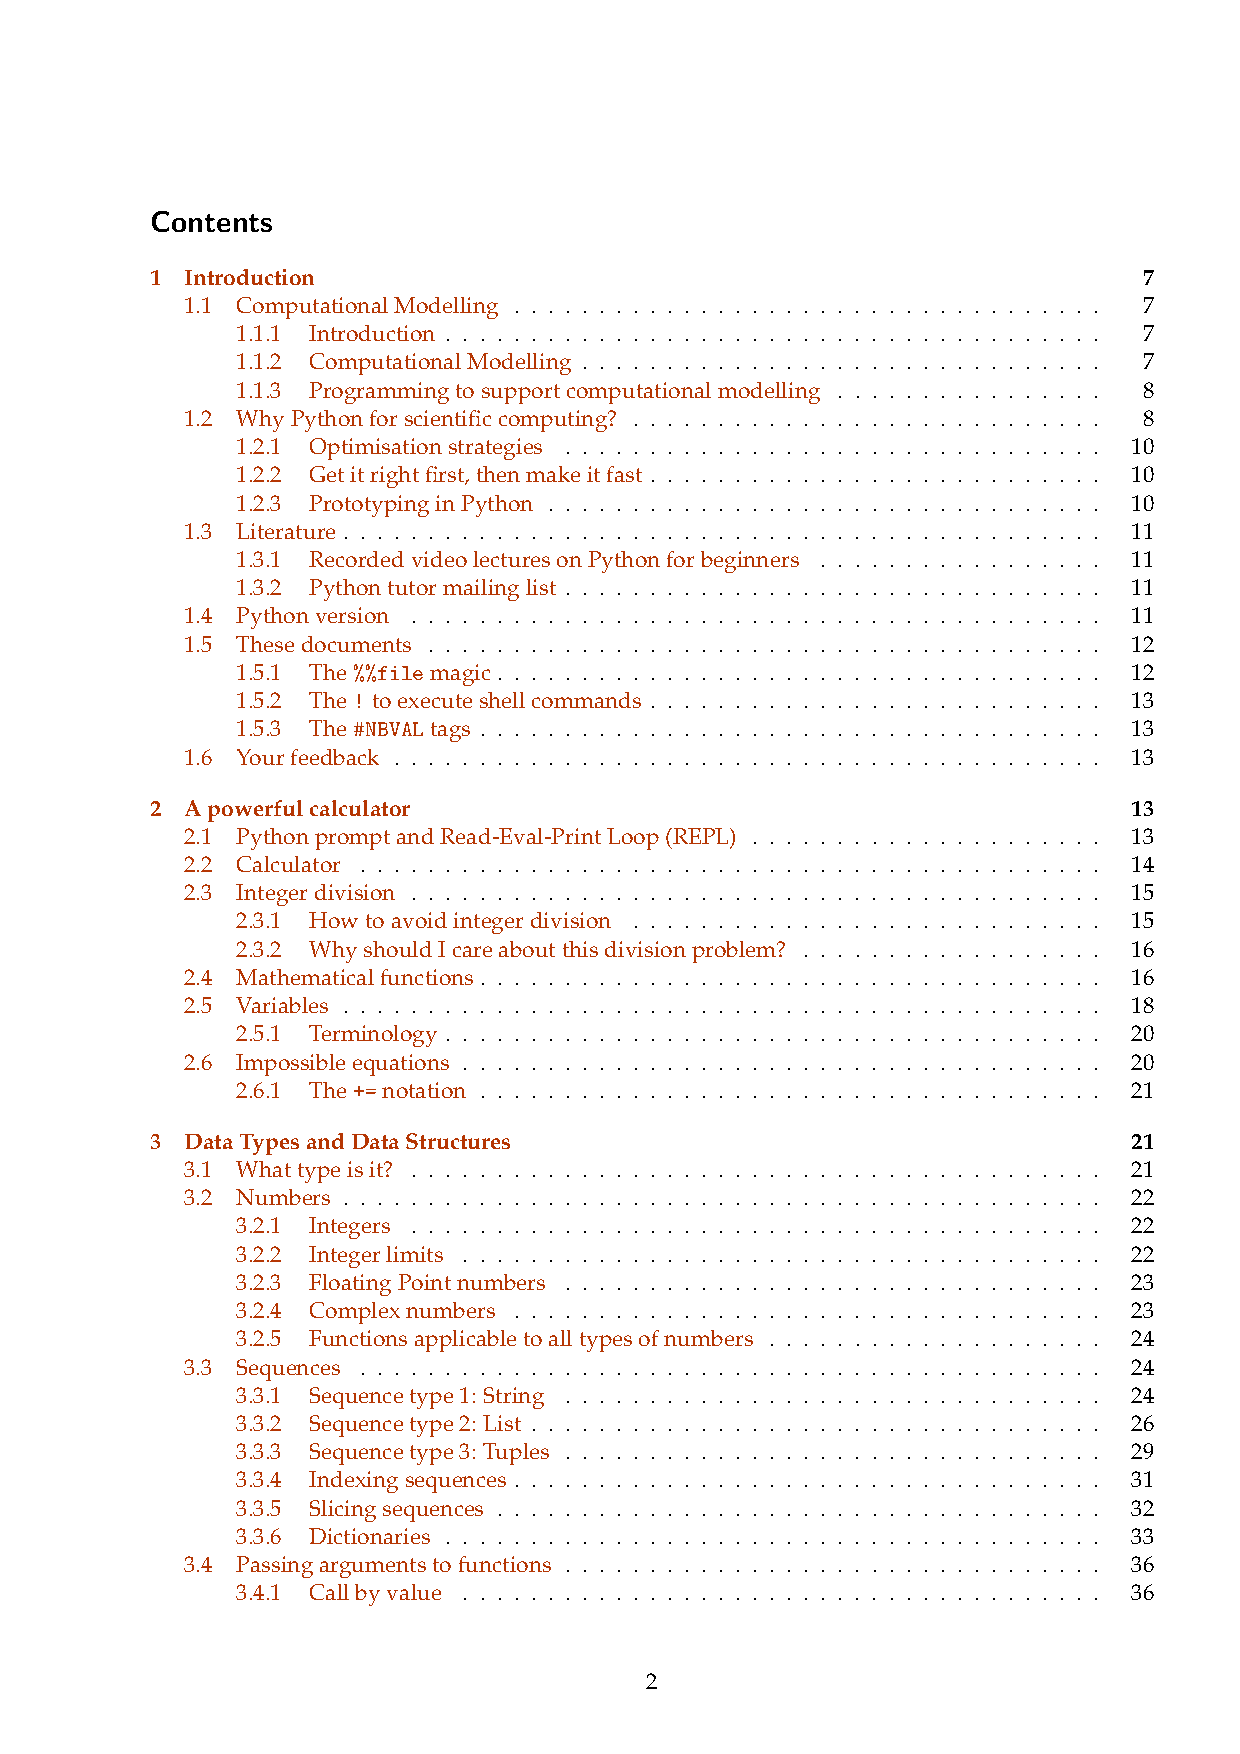
\includepdf[pages={1-5}]{computational-science-table-of-contents.pdf}


\end{document}

%%% Local Variables:
%%% mode: latex
%%% TeX-master: t
%%% End:
